% !TEX TS-program = pdflatex
% !TEX encoding = UTF-8 Unicode

% This is a simple template for a LaTeX document using the "article" class.
% See "book", "report", "letter" for other types of document.

\documentclass[11pt]{article} % use larger type; default would be 10pt

\usepackage[utf8]{inputenc} % set input encoding (not needed with XeLaTeX)

%%% Examples of Article customizations
% These packages are optional, depending whether you want the features they provide.
% See the LaTeX Companion or other references for full information.

%%% PAGE DIMENSIONS
\usepackage{geometry} % to change the page dimensions
\geometry{a4paper} % or letterpaper (US) or a5paper or....
% \geometry{margin=2in} % for example, change the margins to 2 inches all round
% \geometry{landscape} % set up the page for landscape
%   read geometry.pdf for detailed page layout information

\usepackage{graphicx} % support the \includegraphics command and options

% \usepackage[parfill]{parskip} % Activate to begin paragraphs with an empty line rather than an indent

%%% PACKAGES
\usepackage{booktabs} % for much better looking tables
\usepackage{array} % for better arrays (eg matrices) in maths
\usepackage{paralist} % very flexible & customisable lists (eg. enumerate/itemize, etc.)
\usepackage{verbatim} % adds environment for commenting out blocks of text & for better verbatim
\usepackage{subfig} % make it possible to include more than one captioned figure/table in a single float
\usepackage{graphicx}
\usepackage{float}
\usepackage{cite} 
% These packages are all incorporated in the memoir class to one degree or another...

%%% HEADERS & FOOTERS
\usepackage{fancyhdr} % This should be set AFTER setting up the page geometry
\pagestyle{fancy} % options: empty , plain , fancy
\renewcommand{\headrulewidth}{0pt} % customise the layout...
\lhead{}\chead{}\rhead{}
\lfoot{}\cfoot{\thepage}\rfoot{}

%%% SECTION TITLE APPEARANCE
\usepackage{sectsty}
\allsectionsfont{\sffamily\mdseries\upshape} % (See the fntguide.pdf for font help)
% (This matches ConTeXt defaults)

%%% ToC (table of contents) APPEARANCE
\usepackage[nottoc,notlof,notlot]{tocbibind} % Put the bibliography in the ToC
\usepackage[titles,subfigure]{tocloft} % Alter the style of the Table of Contents
\renewcommand{\cftsecfont}{\rmfamily\mdseries\upshape}
\renewcommand{\cftsecpagefont}{\rmfamily\mdseries\upshape} % No bold!

%%% END Article customizations

%%% The "real" document content comes below...

\title{Thesis Draft}

\author{Rubei Riccardo}
%\date{} % Activate to display a given date or no date (if empty),
         % otherwise the current date is printed 

\begin{document}
\maketitle
\newpage
\tableofcontents
\newpage




%Introduction
%% Mention CROSSMINER THe work has been done in that context...

%Mearuring the Similarty of SOftwre Systems
% %You can use some of the content from D6.2. Hopefully, CROSSSim can be included in this section as existing work (saying that it has been developed in the context of CROSSMINER

%Detailed description of the CLAN implementation

%Detailed description of the MUDABlue implementation

% Comparison CROSSSIM,CLAN and MUDABlue, RepoPal
%% Conduct evaluatin on the dataset f 580 Github projects


% Conclusion and Future Work






		\section{Introduction}
		\label{sec:Introduction}
		\subsection{Summary}
Open source software (OSS) repositories contain a large amount of data that has been accumulated along the software development process. Not only source code but also metadata available from different related sources, e.g. communication channels, bug tracking systems, is beneficial to the development process once it is properly mined. Research has been performed to understand and predict software evolution, exploiting the rich metadata available at OSS repositories. This allows for the reduction of effort in knowledge acquisition and quality gain. Developers can leverage the underlying knowledge if they are equipped with suitable tools. For instance, it is possible to empower IDEs by means of tools that continuously monitor the developer's activities and contexts in order to activate dedicated recommendation engines \cite{Ponzanelli:2014:MST:2597073.2597077}. 

%To aim for software quality, for developers it is necessary to understand how similar, mature projects are developed.   it is necessary

To aim for software quality, developers normally build their project by learning from mature OSS projects having comparable functionalities. To this end, the ability to search for similar software projects with respect to different criteria such as functionalities and dependencies plays an important role in the development process. Two projects are deemed to be similar if they implement some features being described by the same abstraction, even though they may contain various functionalities for different domains \cite{McMillan:2012:DSS:2337223.2337267}. Understanding the similarities between open source software projects allows for reusing of source code and prototyping, or choosing alternative implementations \cite{Schafer:2007:CFR:1768197.1768208},\cite{10.1109/SANER.2017.7884605}, thereby improving software quality. Meanwhile measuring the similarities between developers and software projects is a critical phase for most types of recommender systems \cite{DBLP:conf/rweb/NoiaO15},\cite{Sarwar:2001:ICF:371920.372071}. Similarities are used as a base by both content-based and collaborative-filtering recommender systems to choose the most suitable and meaningful items for a given item \cite{Schafer:2007:CFR:1768197.1768208}. Failing to compute precise similarities means concurrently adding a decline in the overall performance of these systems. Nevertheless, measuring similarities between software systems has been considered as a daunting task \cite{Chen:2015:SFD:2684822.2685305},\cite{McMillan:2012:DSS:2337223.2337267}. Furthermore, considering the miscellaneousness of artifacts in open source software repositories, similarity computation becomes more complicated as many artifacts and several cross relationships prevail.

In recent years, considerable effort has been made to provide automated assistance to developers in navigating large information spaces and giving recommendations. Though remarkable progress can be seen in this field, there is still room for improvement. To the best of our knowledge, most of the existing approaches consider the constituent components of the OSS ecosystem separately, without paying much attention to their mutual connections. There is a lack of a proper scheme that facilitates a unified consideration of various OSS artifacts and recommendations. 

CROSSMINER\footnote{\url{https://www.crossminer.org}} is a research project funded by the EU Horizon 2020 Research and Innovation Programme, aiming at supporting the development of complex software systems by \textit{i)} enabling monitoring, in-depth analysis and evidence-based selection of open source components, and \textit{ii)} facilitating knowledge extraction from large OSS repositories \cite{10.1007/978-3-319-74730-9_33}. In the context of the project, we work towards an advanced Eclipse-based IDE providing intelligent recommendations that go far beyond the current \emph{code completion-oriented} practice. Among others, an indispensable functionality is to find a set of similar OSS projects to a given project with respect to different criteria, such as external dependencies, application domain, or API usage \cite{NDRDSEAA2018},\cite{DBLP:conf/iir/NDD013}.

The purpose of this thesis is the implementation of two approaches, MUDABlue and Clan, with the aim of compare the results of new tool by CROSSMINER development team (CrossSim). CROSSSIM (Cross Project Relationships for Computing Open Source Software Similarity), is an approach that makes use of graphs for rep-resenting different kinds of relationships in the OSS ecosystem. In particular, with the adoption of the graph representation, we are able to transform the relationships among non-human artifacts, e.g. API utilizations, source code, interactions, and humans, e.g. developers into a mathematically computable format, i.e. one that
facilitates various types of computation techniques. Naturally this kind of approaches has to be evaluated, and confronted with others similar tools. My work helps addressing this challenge providing these two tools and evaluating all the results to show how nice is CrossSim.
		\clearpage

		\section{The Similarity Problem}
		\label{sec:Similarity}
		\subsection{Overview}

Text similarity measures play an increasingly important role in text related research and applications in tasks such as information retrieval, text classification, document clustering, topic detection, topic tracking, questions generation, question answering, essay scoring, short answer scoring, machine translation, text summarization and others. Finding similarity between words is a fundamental part of text similarity which is then used as a primary stage for sentence, paragraph and document similarities. There two way in which words can be similar each other, lexically if they share sequences of characters similar and  semantically if are used in the same context, used in the same way and so on. 

%%%%%%%%%%%%%%%%%%%%%%%%%%%%%%%%%%%%%%%%%%%%%%%%%%%%%%%%%%

\subsection{String-Based}

The world of lexical similarity con be divided in two categories: character-based and word-based.
To better understand what character-based means, here one of the most well known technique: Levenshtein distance.
\subsubsection{ Levenshtein distance}
 Levenshtein distance defines distance between two strings by counting the minimum number of operations needed to transform one string into the other, where an operation is defined as an insertion, deletion, or substitution of a single character, or a transposition of two adjacent characters.

This is an example:

\begin{itemize}
    \item kitten to sitten (substitution of "s" for "k").
    \item sitten to sittin (substitution of "i" for "e").
    \item sittin to sitting (insertion of "g" at the end).
\end{itemize}

Moving to the word-based,  the word or string similarity measures operate on string sequences and character composition. A string metric is a metric that measures similarity or dissimilarity (distance) between two text strings for approximate string matching or comparison.

\newpage
\subsubsection{Cosine Similarity}

Cosine similarity is a metric used to compute similarity between two objects using their feature vectors \cite{tversky1977features}. An object is characterized as a vector, and for a pair of vectors $\vec{\alpha}=(\alpha_{1},\alpha_{2},..,\alpha_{n})$ and $\vec{\beta}=(\beta_{1},\beta_{2},..,\beta_{n})$ there is an angle between them. Intuitively, the cosine similarity metric measures the similarity as the cosine of the corresponding angle between the two vectors and it is computed using the inner product as follows. 

\begin{equation} \label{eqn:Cosine}
CosineSim(\vec{\alpha},\vec{\beta}) = \frac{\sum_{i=1}^{n}\alpha_{i}\cdot \beta_{i}}{\sqrt{\sum_{i=1}^{n}(\alpha_{i})^{2} }\cdot \sqrt{\sum_{i=1}^{n}(\beta_{i})^{2}}}
\end{equation}

Figure \ref{fig:Cosine} illustrates the cosine similarity between two vectors $\vec{\alpha}$ and $\vec{\beta}$ in a three-dimension space. This can be thought as the similarity between two documents with three terms $t=(t_{1},t_{2},t_{3})$.

\begin{figure}[h!]
	\centering
	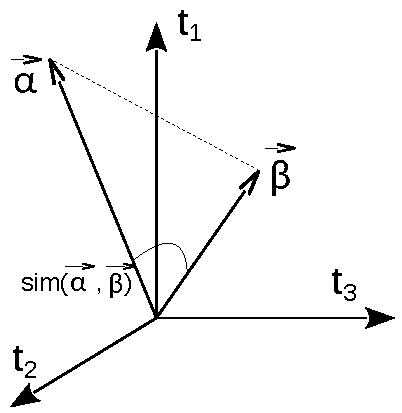
\includegraphics[width=0.25\textwidth]{images/Cosine.pdf}
	\caption{Cosine similarity between two feature vectors $\vec{\alpha}$ and $\vec{\beta}$}
	\label{fig:Cosine}
\end{figure}

Cosine similarity has been popularly adopted in many applications that are related to similarity measurement in various domains \cite{Huang:2012:LCD:2343876.2343884},\cite{Islam:2008:STS:1376815.1376819},\cite{Linden:2003:ARI:642462.642471},\cite{conf:iscis:MadylovaO09},\cite{Mihalcea:2006:CKM:1597538.1597662}. Among the similarity metrics being recalled in this deliverable, the prevalence of Cosine Similarity is obvious as it is utilized in almost all of them as follows: \textit{MUDABlue} \cite{10.1109/APSEC.2004.69}, \textit{CLAN} \cite{McMillan:2012:DSS:2337223.2337267}, \textit{CLANdroid} \cite{10.1109ICPC.2016.7503721}, \textit{LibRec} \cite{6671293}, \textit{SimApp} \cite{Chen:2015:SFD:2684822.2685305}, \textit{WuKong} \cite{Wang:2015:WSA:2771783.2771795}, \textit{TagSim} \cite{Lo:2012:DSA:2473496.2473616}, and \textit{RepoPal} \cite{10.1109/SANER.2017.7884605}.\\

This is an example of how the cosine similarity can be done  between two sentences.
These are the two string that we want to compare to see how much they are related each other.

\begin{itemize}
\item Julie loves me more than Linda loves me.
\item Jane likes me more than Julie loves me.
\end{itemize}
\newpage
From the strings is possible to count the occurrencies of each term, putting everything in a matrix.
\begin{figure}
	\begin{equation} \nonumber
	\bordermatrix{~ & string 1 & string 2 \cr	
		me 		& 2 & 2  \cr 
		Jane		& 0 & 1  \cr  
		Julia		& 1 & 1  \cr
		Linda 		& 1 & 0  \cr 
		likes		& 0 & 1  \cr
		loves		& 2 & 1  \cr
		more		& 1 & 1  \cr
		than		& 1 & 1  \cr	}
	\end{equation}
	\caption{The occurrencies.}
	\label{fig:TDM}
\end{figure}

Since in this kind of evaluation is not important the meaning or where the words are, is possibile to create the related vectore in order to compute the similarity.\\

	\begin{equation} \nonumber
	String1 = [2, 0, 1, 1, 0, 2, 1, 1]
	\end{equation}

	\begin{equation} \nonumber
	String2 = [2, 1, 1, 0, 1, 1, 1, 1]
	\end{equation}

Applying the cosine similarity formula this is the outcome:

\begin{equation} \label{eqn:Cosine}
CosineSim(\vec{\alpha},\vec{\beta}) = \frac{9}{\sqrt{12}\cdot \sqrt{10}} = 0.822
\end{equation}
This means that these strings are close each other 0.822, in a range bewteen 0.0 and 1.0.

%%%%%%%%%%%%%%%%%%%%%%%%%%%%%%%%%%%%%%%%%%%%%%%%%%%%%%%%%%  
\subsection{Corpus-Based}
\subsubsection{Term-Document Matrix}
 In Natural Language Processing \cite{Collobert:2011:NLP:1953048.2078186}, a term-document matrix (TDM) is used to represent the relationships between words and documents \cite{Turney:2010:FMV:1861751.1861756}. In a TDM, each row corresponds to a document and each column corresponds to a term. A cell in the TDM represents the weight of a term in a document. The most common weighting scheme used in document retrieval is the \emph{term frequency-inverse document frequency (tf-idf)} function \cite{Reed:2006:TNT:1193211.1193734}. If we consider a set of $n$ documents $D=(d_{1},d_{2},..,d_{n})$ and a set of terms $t=(t_{1},t_{2},..,t_{r})$ then the representation of a document $d \in D $ is vector $\vec{\delta}=(w_{1}^{d},w_{2}^{d},..,w_{r}^{d})$, where the weight $w_{k}^{d}$ of term $k$ in document $d$ is computed using the {\em tf-idf} function \cite{Ramos1999}:

\begin{equation} \label{tfidf} %\nonumber 
w_{k}^{d} =tf\cdot idf(k,d,D)= f_{k}^{d}\cdot log\frac{n}{\left | \left \{ d\in D: t_{k} \in d \right \} \right |} 
\end{equation}

where $f_{k}^{d}$ is the frequency of term $t_{k}$ in document $d$.

Another common weighting scheme uses only the frequency of terms in documents for cells in TDM, i.e. the number of occurrence of a term in a document, instead of {\em tf-idf}. As an example, we consider a set of three simple documents $D=(d_{1},d_{2},d_{3})$ as follows:

\begin{itemize}
	\item[+] $d_{1}$: \emph{She is nice.}
	\item[+] $d_{2}$: \emph{Today is nice.}
	\item[+] $d_{3}$: \emph{Nice is a nice city.}
\end{itemize}

\begin{figure}[h!]
	\begin{equation} \nonumber
	\bordermatrix{~ & she & is & today & a & nice & city \cr	
		d_{1} 		& 1 & 1 & 0 & 0 & 1 & 0 \cr 
		d_{2} 		& 0 & 1 & 1 & 0 & 1 & 0 \cr  
		d_{3} 		& 0 & 1 & 0 & 1 & 2 & 1 \cr }
	\end{equation}
	\caption{An example of a term-document matrix}
	\label{fig:TDM}
\end{figure}

The set of terms $t$ consists of $6$ elements, i.e. $t=(she$, $is$, $today$, $a$, $nice$, $city)$ and the corresponding term-document matrix for $D$ is depicted in Figure \ref{fig:TDM}.

TDM has been exploited to characterize software systems and finally to compute similarities between them \cite{10.1109/APSEC.2004.69},\cite{10.1109ICPC.2016.7503721},\cite{McMillan:2012:DSS:2337223.2337267}. In a TDM for software systems, each row represents a package, an API call or a function and each column represents a software system. A cell in the matrix is the number of occurrence of a package/an API/function in each corresponding software system. A TDM for software systems has a similar form to the matrix shown in Figure \ref{fig:TDM} where documents are replaced by software systems and terms are replaced by API calls.

\subsubsection{Latent Semantic Analysis}

The problem with the term-document matrix is that the intrinsic relationships among different terms of a document cannot fully be captured. Furthermore, same words can be used to explain different requirements or the other way around, the same requirements can be described using different words \cite{10.1109/APSEC.2004.69}. Latent Semantic Analysis (LSA), also known as Latent Semantic Indexing (LSI), has been proposed to overcome these problems \cite{Landauer1998}. The technique exploits a mathematical model that can infer latent semantic relationships to compute similarity. LSA represents the contextual usage meaning of words by statistical computations applied to a large corpus of text. It then generates a representation that captures the similarity of words and text passages. To perform LSA on a text, a term-document matrix is created to characterize the text. Afterwards, Singular Value Decomposition (SVD) - a matrix decomposition technique - is used in combination with LSA to reduce matrix dimensionality \cite{kb2005}. SVD takes a highly variable set of data entries as input and transforms to a lower dimensional space but reveals the substructure of the original data. Essentially, it decomposes a rectangular matrix into the product of three other matrices as given below\cite{kb2005}:

\begin{equation}
A_{mn}=U_{mm}S_{mn}V_{mn}^{T}
\end{equation}

in which

\begin{itemize}
	\item $U_{mm}$: Orthogonal matrix.
	\item $S_{mn}$: Diagonal matrix.
	\item $V_{mn}^{T}$: The transpose of an orthogonal matrix.
	\item $X$: Low Rank matrix.
\end{itemize}


$U_{mm}$ describes the original row entities as vectors of derived orthogonal factor values. $S_{mn}$ represents the original column entities in the same way, and $V_{mn}$ is a diagonal matrix containing scaling values. With the application of LSA it is possible to find the most relevant features and remove the least important ones by means of the reduced matrix $U_{mm}$. As a result, an equivalence of $A_{mm}$ can be constructed using the most relevant features. LSA helps reveal the latent relationship among words as well as among passages which cannot be guaranteed by a simple term-document matrix. The similarity measurement by LSA reflects adequately human perception of similarity and association among texts. Using LSA, similarities among documents are measured as the cosine of the angle between their row vectors (see Sec. \ref{sec:cosine}). LSA has been applied in \cite{10.1109/APSEC.2004.69},\cite{10.1109ICPC.2016.7503721},\cite{McMillan:2012:DSS:2337223.2337267} to compute similarities of software systems. The main disadvantage of LSA is that it is computational expensive when a large amount of information is analyzed.

\newpage

An example.
Image that these are a set of document to be analyzed and we want to apply the procedure stated before.
\begin{itemize}
	\item doc1: Human machine interface for ABC computer applications
	\item doc2: A survey of user opinion of computer system response time
	\item doc3: The EPS user interface management system
	\item doc4: System and human system engineering testing of EPS
	\item doc5: Relation of user perceived response time to error measurement
	\item doc6: The generation of random, binary, ordered trees
	\item doc7: The intersection graph of paths in trees
	\item doc8: Graph minors IV: Widths of trees and well-quasi-ordering
	\item doc9: Graph minors: A survey
\end{itemize}

\begin{figure}[h!]
	\begin{equation} \nonumber
	\bordermatrix{~ & doc1 & doc2 & doc3 & doc4 & doc5 & doc6 & doc7 & doc8 & doc9 \cr	
		human	& 1 & 0 & 0 & 1 & 0 & 0 & 0 & 0 & 0 \cr
		interface	& 1 & 0 & 1 & 0 & 0 & 0 & 0 & 0 & 0 \cr
		computer	& 1 & 1 & 0 & 0 & 0 & 0 & 0 & 0 & 0 \cr    
		user 		& 0 & 1 & 1 & 0 & 2 & 0 & 0 & 0 & 0 \cr
		system 	& 0 & 1 & 1 & 2 & 0 & 0 & 0 & 0 & 0 \cr
		response	& 0 & 1 & 0 & 0 & 1 & 0 & 0 & 0 & 0 \cr
		time 		& 0 & 0 & 1 & 1 & 0 & 0 & 0 & 0 & 0 \cr
		EPS 		& 0 & 1 & 0 & 0 & 0 & 0 & 0 & 0 & 1 \cr
		survey	& 0 & 0 & 0 & 0 & 0 & 1 & 1 & 1 & 0 \cr
		trees 		& 0 & 0 & 0 & 0 & 0 & 0 & 1 & 1 & 1 \cr
		graph 		& 0 & 0 & 0 & 0 & 0 & 0 & 0 & 1 & 1 \cr
		minors		& 1 & 1 & 0 & 0 & 1 & 0 & 1 & 1 & 0 \cr	  }
	\end{equation}
	\caption{Term-Document matrix related to the example.}
	\label{fig:TDM}
\end{figure}

\begin{figure}[h!]
	\begin{equation} \nonumber
	\bordermatrix{ ~ \cr
		& 0.22 & -0.11 & 0.29 & -0.41 & -0.11 & -0.34 & 0.52 & -0.06 & -0.41 \cr
		& 0.20 & -0.07 & 0.14 & -0.55 & 0.28 & 0.50 & -0.07 & -0.01 & -0.11 \cr
		& 0.24 & 0.04 & -0.16 & -0.59 & -0.11 & -0.25 & -0.30 & 0.06 & 0.49 \cr
		& 0.40 & 0.06 & -0.34 & 0.10 & 0.33 & 0.38 & 0.00 & 0.00 & 0.01 \cr
		& 0.64 & -0.17 & 0.36 & 0.33 & -0.16 & -0.21 & -0.17 & 0.03 & 0.27 \cr
		& 0.27 & 0.11 & -0.43 & 0.07 & 0.08 & -0.17 & 0.28 & -0.02 & -0.05 \cr
		& 0.27 & 0.11 & -0.43 & 0.07 & 0.08 & -0.17 & 0.28 & -0.02 & -0.05 \cr
		& 0.30 & -0.14 & 0.33 & 0.19 & 0.11 & 0.27 & 0.03 & -0.02 & -0.17 \cr
		& 0.21 & 0.27 & -0.18 & -0.03 & -0.54 & 0.08 & -0.47 & -0.04 & -0.58 \cr
		& 0.01 & 0.49 & 0.23 & 0.03 & 0.59 & -0.39 & -0.29 & 0.25 & -0.23 \cr
		& 0.04 & 0.62 & 0.22 & 0.00 & -0.07 & 0.11 & 0.16 & -0.68 & 0.23 \cr
		& 0.03 & 0.45 & 0.14 & -0.01 & -0.30 & 0.28 & 0.34 & 0.68 & 0.18 \cr	  }
	\end{equation}
	\caption{$U_{mm}$x}
	\label{fig:TDM}
\end{figure}

\begin{figure}[h!]
	\begin{equation} \nonumber
	\bordermatrix{~  \cr	
		& 3.34 & 0 & 0 & 0 & 0 & 0 & 0 & 0 & 0 \cr
		& 0 & 2.54 & 0 & 0 & 0 & 0 & 0 & 0 & 0 \cr
		& 0 & 0 & 2.35 & 0 & 0 & 0 & 0 & 0 & 0 \cr
		& 0 & 0 & 0 & 1.64 & 0 & 0 & 0 & 0 & 0 \cr
		& 0 & 0 & 0 & 0 & 1.50 & 0 & 0 & 0 & 0 \cr
		& 0 & 0 & 0 & 0 & 0 & 1.31 & 0 & 0 & 0 \cr
		& 0 & 0 & 0 & 0 & 0 & 0 & 0.85 & 0 & 0 \cr
		& 0 & 0 & 0 & 0 & 0 & 0 & 0 & 0.56 & 0 \cr
		& 0 & 0 & 0 & 0 & 0 & 0 & 0 & 0 & 0.36 \cr
	  }
	\end{equation}
	\caption{ $S_{mn}$}
	\label{fig:TDM}
\end{figure}

\clearpage
\begin{figure}[h!]
	\begin{equation} \nonumber
	\bordermatrix{~  \cr	
		& 0.20 & 0.61 & 0.46 & 0.54 & 0.28 & 0.00 & 0.01 & 0.02 & 0.08 \cr
		& -0.06 & 0.17 & -0.13 & -0.23 & 0.11 & 0.19 & 0.44 & 0.62 & 0.53 \cr
		& 0.11 & -0.50 & 0.21 & 0.57 & -0.51 & 0.10 & 0.19 & 0.25 & 0.08 \cr
		& -0.95 & -0.03 & 0.04 & 0.27 & 0.15 & 0.02 & 0.02 & 0.01 & -0.03 \cr
		& 0.05 & -0.21 & 0.38 & -0.21 & 0.33 & 0.39 & 0.35 & 0.15 & -0.60 \cr
		& -0.08 & -0.26 & 0.72 & -0.37 & 0.03 & -0.30 & -0.21 & 0.00 & 0.36 \cr
		& 0.18 & -0.43 & -0.24 & 0.26 & 0.67 & -0.34 & -0.15 & 0.25 & 0.04 \cr
		& -0.01 & 0.05 & 0.01 & -0.02 & -0.06 & 0.45 & -0.76 & 0.45 & -0.07 \cr
		& -0.06 & 0.24 & 0.02 & -0.08 & -0.26 & -0.62 & 0.02 & 0.52 & -0.45 \cr	 
 }
	\end{equation}
	\caption{$V_{mn}^{T}$}
	\label{fig:TDM}
\end{figure}
The following image depict the result of the decomposition with a rank of 2.
\begin{table}[h!]
	\begin{equation} \nonumber
	\bordermatrix{~ & doc1 & doc2 & doc3 & doc4 & doc5 & doc6 & doc7 & doc8 & doc9 \cr	
		human 	& 0.16 & 0.40 & 0.38 & 0.47 & 0.18 & -0.05 & -0.12 & -0.16 & -0.09 \cr
		interface 	& 0.14 & 0.37 & 0.33 & 0.40 & 0.16 & -0.03 & -0.07 & -0.10 & -0.04 \cr
		computer	& 0.15 & 0.51 & 0.36 & 0.41 & 0.24 & 0.02 & 0.06 & 0.09 & 0.12 \cr
		user 		& 0.26 & 0.84 & 0.61 & 0.70 & 0.39 & 0.03 & 0.08 & 0.12 & 0.19 \cr
		system 	& 0.45 & 1.23 & 1.05 & 1.27 & 0.56 & -0.07 & -0.15 & -0.21 & -0.05 \cr
		response 	& 0.16 & 0.58 & 0.38 & 0.42 & 0.28 & 0.06 & 0.13 & 0.19 & 0.22 \cr
		time 		& 0.16 & 0.58 & 0.38 & 0.42 & 0.28 & 0.06 & 0.13 & 0.19 & 0.22 \cr
		EPS 	 	& 0.22 & 0.55 & 0.51 & 0.63 & 0.24 & -0.07 & -0.14 & -0.20 & -0.11 \cr 
		survey 	& 0.10 & 0.53 & 0.23 & 0.21 & 0.27 & 0.14 & 0.31 & 0.44 & 0.42 \cr
		trees 		& -0.06 & 0.23 & -0.14 & -0.27 & 0.14 & 0.24 & 0.55 & 0.77 & 0.66 \cr
		graph 		& -0.06 & 0.34 & -0.15 & -0.30 & 0.20 & 0.31 & 0.69 & 0.98 & 0.85 \cr
		minors 	& -0.04 & 0.25 & -0.10 & -0.21 & 0.15 & 0.22 & 0.50 & 0.71 & 0.62 \cr	  }
	\end{equation}
	\caption{Matrix decomposed.}
	\label{fig:TDM}
\end{table}
\clearpage

\begin{figure}[h!]
	\centering
	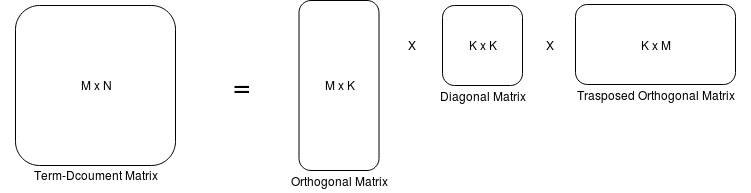
\includegraphics[width=15cm,height=20cm,keepaspectratio]{images/LSIk.png}
	\caption{Reduction phase}
	\label{fig:LSIk}
\end{figure}

Figure \ref{fig:LSIk} depicts the low rank reduction phase and is interesting to graphically see what does it mean. The new matrix is the product of the other three, but reducted, this is a very relevant issue. If the singular values in $S_{mn}$ are ordered by size, the first k largest may be kept and the remaining smaller ones set to zero. The product of the resulting matrices is a matrix $X$ which is only approximately equal to $A_{mm}$ , and is of rank k . It can be shown that the new matrix $X$ is the matrix of rank k which is closest in the least squares sense to $A_{mm}$ .
The amount of dimension reduction, i.e., the choice of k , is critical to our work. Ideally, we want a value of k that is large enough to fit all the real structure in the data, but small enough so that we do not also fit the sampling error or unimportant details. The proper way to make such choices is an open issue in the factor analytic literature. In practice, we currently use an operational criterion - a value of k which yields good retrieval performance.\\ In our work we decided a \emph{k value =} $\frac{repository}{2}$

\clearpage
%%%%%%%%%%%%%%%%%%%%%%%%%%%%%%%%%%%%%%%%%%%%%%%%%%%%%%%%%%  
\subsection{Knowledge-Based}
Knowledge-Based Similarity aims to identify the degree of similarity between words using informations derived from semantic networks.
Knowledge-based similarity measures can be divided roughly into two groups: measures of semantic similarity and measures of semantic relatedness.By semantic similarity we mean concepts that are related each other on the basis of their likeness.
Semantic relatedness, on the other hand, is a more general notion of relatedness, not specifically tied to the shape or form of the concept. Semantic similarity is a metric defined over a set of documents or terms, where the idea of distance between them is based on the likeness of their meaning or semantic content as opposed to similarity which can be estimated regarding their syntactical representation (e.g. their string format).
An example of relatedness is the Lask algorithm which identify senses of words in context using definition overlap. To clarify let's take a look an example in \cite{Resnik}.
Using the Oxford Advanced Learner's Dictionary, it finds that word \emph{pine} has two senses:
\begin{itemize}
	\item{Sense 1: kind of \textbf{evergreen tree} with needle-shaped leaves}
	\item{Sense 2: waste away through sorrow ir illness.}
\end{itemize}

The word \emph{cone} has three senses:
\begin{itemize}
	\item{Sense 1: solid body which narrows to a point}
	\item{Sense 2: something of this shape whether solid or hollow}
	\item{Sense 3: fruit of certain \textbf{evergreen tree}}
\end{itemize}

Each of the two senses of the word \emph{pine} is compared with each of the three senses of the \emph{cone} and it is found that the words \emph{evergreen tree} occurs in one sense each of the two words. These two senses are then declared to be the most appropriate senses when words \emph{pine} and \emph{cone} are used togheter.

Concerning the similarity an example could be Resnik(1995) which uses the information content of concepts, computed from their frequency of occurrence in a large corpus, to determine the semantic relatedness of word senses\cite{Resnik}.
Another example is Jian \& Conrath \cite{Jian}s It combines a lexical taxonomy structure with corpus statistical information so that the semantic distance between nodes in the semantic space constructed by the taxonomy can be better quantified with the computational evidence derived from a distributional analysis of corpus data. Specifically, the proposed measure is a combined approach that inherits the edge-based approach of the edge counting scheme, which is then enhanced by the node-based approach of the information content calculation.

		\clearpage

		\section{The Approaches}
		\label{sec:Approaches}
		%%%%%%%%%%%%%%%%%%%%%%%%%%%%%%%%%%%%%%%%%%%%%%%%%%%%%%%%%%

\subsection{MUDABlue}\label{sec:mudablue}

The first procedure analysed was MUDABlue, unfortunately none implentation was available on the web, so i reimplemented it from scratch. The MUDABlue method is an automatc categorizaton method or a large collecton of software systems. MUDABlue method does not only categorize sooware systemsd but also determines categories rom the sooware systems collecton automatcally. MUDABlue has three major aspects: 1) it relies on no other information than the source code, 2) it determines category sets automatically, and 3) it allows a software system to be a member of multiple categories. Since we were interested only in the evaluation of the similarity we discarded the phases related to clusterization and categorization.

\subsection{The Approach}

The MUDABlue approach can be briefly summarized in 7 steps, as the following image depicts:

\begin{figure}[H]
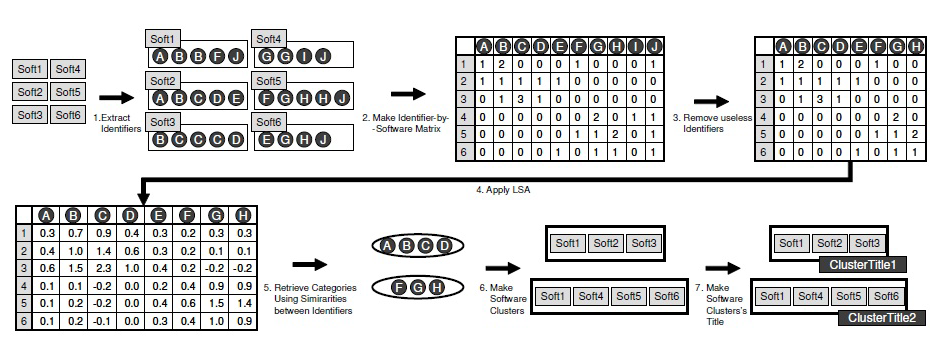
\includegraphics[width=15cm,height=20cm,keepaspectratio]{images/Mudablue1.png}
\centering
\caption{MUDABlue phases.}
\end{figure}

\subsubsection{Exctract Identifiers}
With identifier we are talking about relevant strings that can allow to characterize a document. In this phase each repository is scanned in order to find the target files, and for each of them the identifiers are exctracted, avoiding adding useless items such as comments. The dataset was a 41C projects gathered from SourceForge.

\subsubsection{Create identifier-by-software matrix}
As stated before, the main item to work with is the term-document matrix, in this case we count how many times each term appears in each file for all the projects. The result is matrix \textbf{m x n} with m terms and n projects.

\subsubsection{Remove useless identifiers}
From the matrix we remove all the useless terms, that is all the terms that apperas in just one repository, considered a specific terms, and all the terms that appears in more than 50\% of the repositories, considered as general terms.

\subsubsection{Apply the LSA}
Once the matrix is ready con be worked, the SVD procedure is applied and then the LSI. As explained before [NOTE] the SVD procedure decompose the original matrix in 3 other matrices. When we multiply back these matrices we use a rank reducted version of the S matrix in order to generete the final one. The authors didn't provide us any details about their final rank value, so we tested many values and eventually selected one.

\subsubsection{Apply the Cosine Similarity}
By using the cosine similarity method, we compare each repository vector with all the others and eventually getting an \textbf{n x n} matrix, in which is expressed the similarity of all the repository couple, with a value [0.0-1.0].

\subsubsection{Categorization}
The point 6 and 7 are not covered because not related to our work.
\clearpage



%%%%%%%%%%%%%%%%%%%%%%%%%%%%%%%%%%%%%%%%%%%%%%%%%%%%%%%%%%

\subsection{CLAN:  Closely reLated ApplicatioNs}\label{sec:clan}

\textit{CLAN} \cite{McMillan:2012:DSS:2337223.2337267} is an approach for automatically detecting similar Java applications by exploiting the semantic layers corresponding to packages class hierarchies. \textit{CLAN} works based on the document framework for computing similarity, semantic anchors, e.g. those that define the documents' semantic features. Semantic anchors and dependencies help obtain a more precise value for similarity computation between documents. The assumption is that if two applications have API calls implementing requirements described by the same abstraction, then the two applications are more similar than those that do not have common API calls. The approach uses API calls as semantic anchors to compute application similarity since API calls contain precisely defined semantics. The similarity between applications is computed by matching the semantics already expressed in the API calls.

\subsection{The Approach}

The process consist of 12 steps here graphically reported.

\begin{figure}[H]
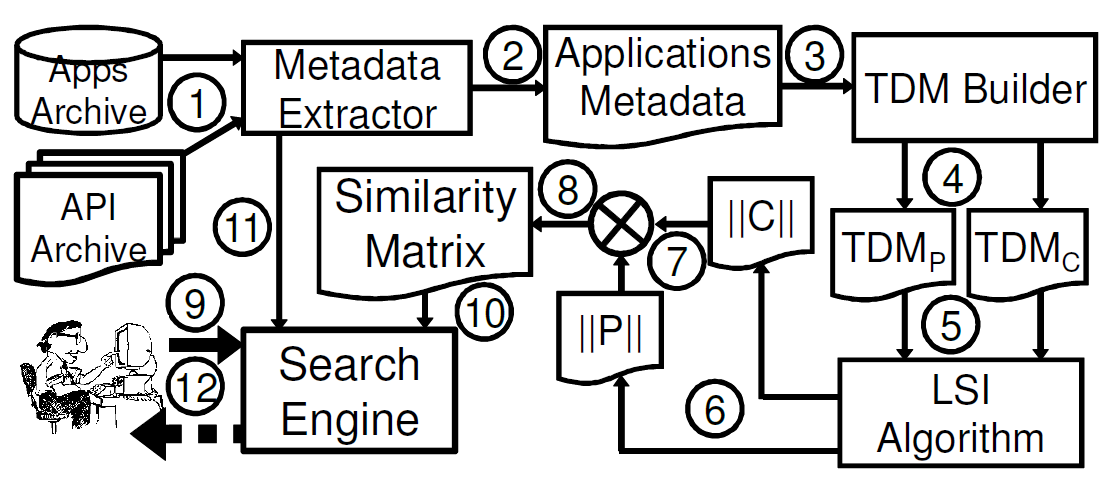
\includegraphics[width=15cm,height=20cm,keepaspectratio]{images/Clan.png}
\centering
\caption{CLAN phases.}
\end{figure}

\subsubsection{1 - 3: Terms Extraction}
Steps from 1 to 3 can be merged together since are related to extraction of terms from the repositories.
As stated before, an important concept is that terms extracted are only API calls, this means that all other things present in a piece of code are discarded, for example all the variables or the function declaration and invocation. Furthermore these API calls belong only to the JDK, in such a way also the calls to any other external library are discarded. This idea is also applied in the extraction of the import declaration, focus only on the JDK packages import.
The result of this process will be an ordered set of data, representing the occurrencies of any Package;Class for all the projects.

\subsubsection{4: TDMs Creation}
Once the dataset as been created, is reorganized in TDMs. Here two different matrices are created, one for the Classes and one for the Packages. Class-level and package-level similarities are different since applications are often more similar on the package level than on the class level because there are fewer packages than classes in the JDK. Therefore, there is the higher probability that two applications may have API calls that are located in the same package but not in the same class.

\subsubsection{5: LSI Procedure}

\subsubsection{6: Apply the Cosine Similarity}

\subsubsection{7: Sum of the matrices}
The 2 matrices are summed, but before are multplied by a certain value. Since the values for the entries in the 2 matrices are between 0.0 and 1.0 a simple sum could result in a value over 1.0, by this multiplication these values are reducted in order to be summed togheter but still maintaining the logical meaning. The authors chosen 0.5, also we, since is a good value to equal distribute the weight of the packages and method calls.The sum of this value is 1.0, and can span from 0.1 to 0.9 for each matrix, is clear that more is high on a matrix, more is important the values that we are considering from such matrix.

\subsubsection{8: Final similarity matrix}
\clearpage


%%%%%%%%%%%%%%%%%%%%%%%%%%%%%%%%%%%%%%%%%%%%%%%%%%%%%%%%%%  

\subsubsection{RepoPal: Exploiting Metadata to Detect Similar GitHub Repositories}\label{sec:repopal}

In contrast to many previous studies that are generally based on source code \cite{10.1109/APSEC.2004.69},\cite{Liu:2006:GDS:1150402.1150522},\cite{McMillan:2012:DSS:2337223.2337267}, \textit{RepoPal}  \cite{10.1109/SANER.2017.7884605} is a high-level similarity metric and takes only repositories metadata as its input. With this approach, two GitHub repositories are considered to be similar if:

\begin{itemize}
	\item[i)] They contain similar readme files;
	\item[ii)] They are starred by users of similar interests;
	\item[iii)] They are starred together by the same users within a short period of time. 
\end{itemize}

Thus, the similarities between GitHub repositories are computed by using three inputs: readme file, stars and the time gap that a user stars two repositories. Considering two repositories $ r_{i} $ and $ r_{j} $, the following notations are defined: 

\begin{itemize}
	\item $ f_{i} $ and $ f_{j} $ are the readme files with $ t $ being the set of terms in the files; 
	\item $ U(r_{i}) $ and $ U(r_{j}) $ are the set of users who starred $ r_{i} $ and $ r_{j} $, respectively; 
	\item $ R(u_{k}) $ is the set of repositories that user $ u_{k} $ already starred.  
\end{itemize}

There are three similarity indices as follows:

\paragraph{Readme-based similarity} 

The similarity between two readme files is calculated as the cosine similarity between their feature vectors $\vec{f_{i}}$ and $\vec{f_{j}}$: 

\begin{equation}
sim_{f}(r_{i},r_{j})=CosineSim(\vec{f_{i}},\vec{f_{j}})
\end{equation}
		\clearpage


		\bibliographystyle{plain}
		\bibliography{ThesisDraft}

\end{document}
